\documentclass[10pt,sigconf,letterpaper,anonymous]{acmart}

\usepackage{algorithmic}
\usepackage{algorithm}

\usepackage[english]{babel}
\usepackage{blindtext}

%% These commands are for a PROCEEDINGS abstract or paper.
\acmConference{CoNEXT '19}{December 9-12, 2019}{Orlando, Florida, USA}

%% Rights management information.  This information is sent to you
%% when you complete the rights form.  These commands have SAMPLE
%% values in them; it is your responsibility as an author to replace
%% the commands and values with those provided to you when you
%% complete the rights form.
\setcopyright{acmcopyright}
\copyrightyear{2019}
\acmYear{2019}
% \acmDOI{10.1145/1122445.1122456}

%% These commands are for a PROCEEDINGS abstract or paper.
%L: These will be provided later
%\acmConference[Conext'19]{}{}{}
%\acmBooktitle{}
%\acmPrice{}
%\acmISBN{}
% User Defined Commands
\settopmatter{printacmref=false}
\newcommand{\ggx}[1]{\textcolor{cyan}{[L: #1]}}
\newcommand{\vk}[1]{\textcolor{red}{[V: #1]}}

%\newcommand{\ggx}[1]{}
%\newcommand{\vk}[1]{}



\begin{document}

%%
%% The "title" command has an optional parameter,
%% allowing the author to define a "short title" to be used in page headers.
\title{A Fair Packet Drop Algorithm for Deterministic Networks (Detnet)}
\subtitle{Paper \#205, 6 pages}
%%
%% The "author" command and its associated commands are used to define
%% the authors and their affiliations.
%% Of note is the shared affiliation of the first two authors, and the
%% "authornote" and "authornotemark" commands
%% used to denote shared contribution to the research.
\author{Vamsi Addanki}
\email{vaddanki@telecom-paristech.fr}
\affiliation{%
  \institution{Telecom Paristech}
  \streetaddress{23 Avenue d'italie}
  \city{Paris}
  \state{France}
  \postcode{75013}
}

\author{Luigi Iannone}
\email{luigi.iannone@telecom-paristech.fr}
\affiliation{%
  \institution{Telecom Paristech}
  \streetaddress{23 Avenue d'italie}
  \city{Paris}
  \state{France}
  \postcode{75013}
}


%%
%% By default, the full list of authors will be used in the page
%% headers. Often, this list is too long, and will overlap
%% other information printed in the page headers. This command allows
%% the author to define a more concise list
%% of authors' names for this purpose.
\renewcommand{\shortauthors}{Addanki et al.}

%%
%% The abstract is a short summary of the work to be presented in the
%% article.
\begin{abstract}
 The Internet works as a best-effort service, without guarantees. The end-to-end latency, jitter and packet-loss probability have no fixed bounds. However, there is a fast-growing demand, in the context of industrial use-cases, for the so-called \emph{Deterministic Networks} (DetNet). DetNets are a special implementation of protocol stack, where thanks to bandwidth reservation, priority-based queuing, and traffic replication, latency can be bounded and packet-loss is avoided. In this paper, we propose a modified fair drop algorithm, able to prioritize packets so that a DetNet flow can fully use its reserved bandwidth without any interference from other flows, while at the same time allowing best-effort traffic to take advantage of reserved but unused bandwidth. We implemented such algorithm in NS3 and show how we meet the DetNet requirements. We mainly
focused on bandwidth reservation part of deterministic networks. 
We aim at zero congestion loss for priority flows by
bandwidth reservation, and fair usage of unreserved and/or total unused bandwidth for non-priority flows. In contrary to the idea of increasing number of buffers to reduce the probability of packet loss, we show that the algorithm we adopt can achieve zero packet loss with only one shared buffer for all flows in our experiments.
\end{abstract}

%%
%% The code below is generated by the tool at http://dl.acm.org/ccs.cfm.
%% Please copy and paste the code instead of the example below.
%%
%\begin{CCSXML}
%<ccs2012>
% <concept>
%  <concept_id>10010520.10010553.10010562</concept_id>
%  <concept_desc>Computer systems organization~Embedded systems</concept_desc>
%  <concept_significance>500</concept_significance>
% </concept>
% <concept>
%  <concept_id>10010520.10010575.10010755</concept_id>
%  <concept_desc>Computer systems organization~Redundancy</concept_desc>
%  <concept_significance>300</concept_significance>
% </concept>
% <concept>
%  <concept_id>10010520.10010553.10010554</concept_id>
%  <concept_desc>Computer systems %organization~Robotics</concept_desc>
%  <concept_significance>100</concept_significance>
% </concept>
% <concept>
%  <concept_id>10003033.10003083.10003095</concept_id>
% <concept_desc>Networks~Network reliability</concept_desc>
%  <concept_significance>100</concept_significance>
% </concept>
%</ccs2012>
%end{CCSXML}

%\ccsdesc{Network Algorithms}
%\ccsdesc{Traffic Engineering}
%\ccsdesc{Bandwidth Reservation}
%\ccsdesc{Deterministic Networks}

%%
%% Keywords. The author(s) should pick words that accurately describe
%% the work being presented. Separate the keywords with commas.
%\keywords{Deterministic Network; Algorithms; Bandwidth reservation;}

%% A "teaser" image appears between the author and affiliation
%% information and the body of the document, and typically spans the
%% page.
% \begin{teaserfigure}
%   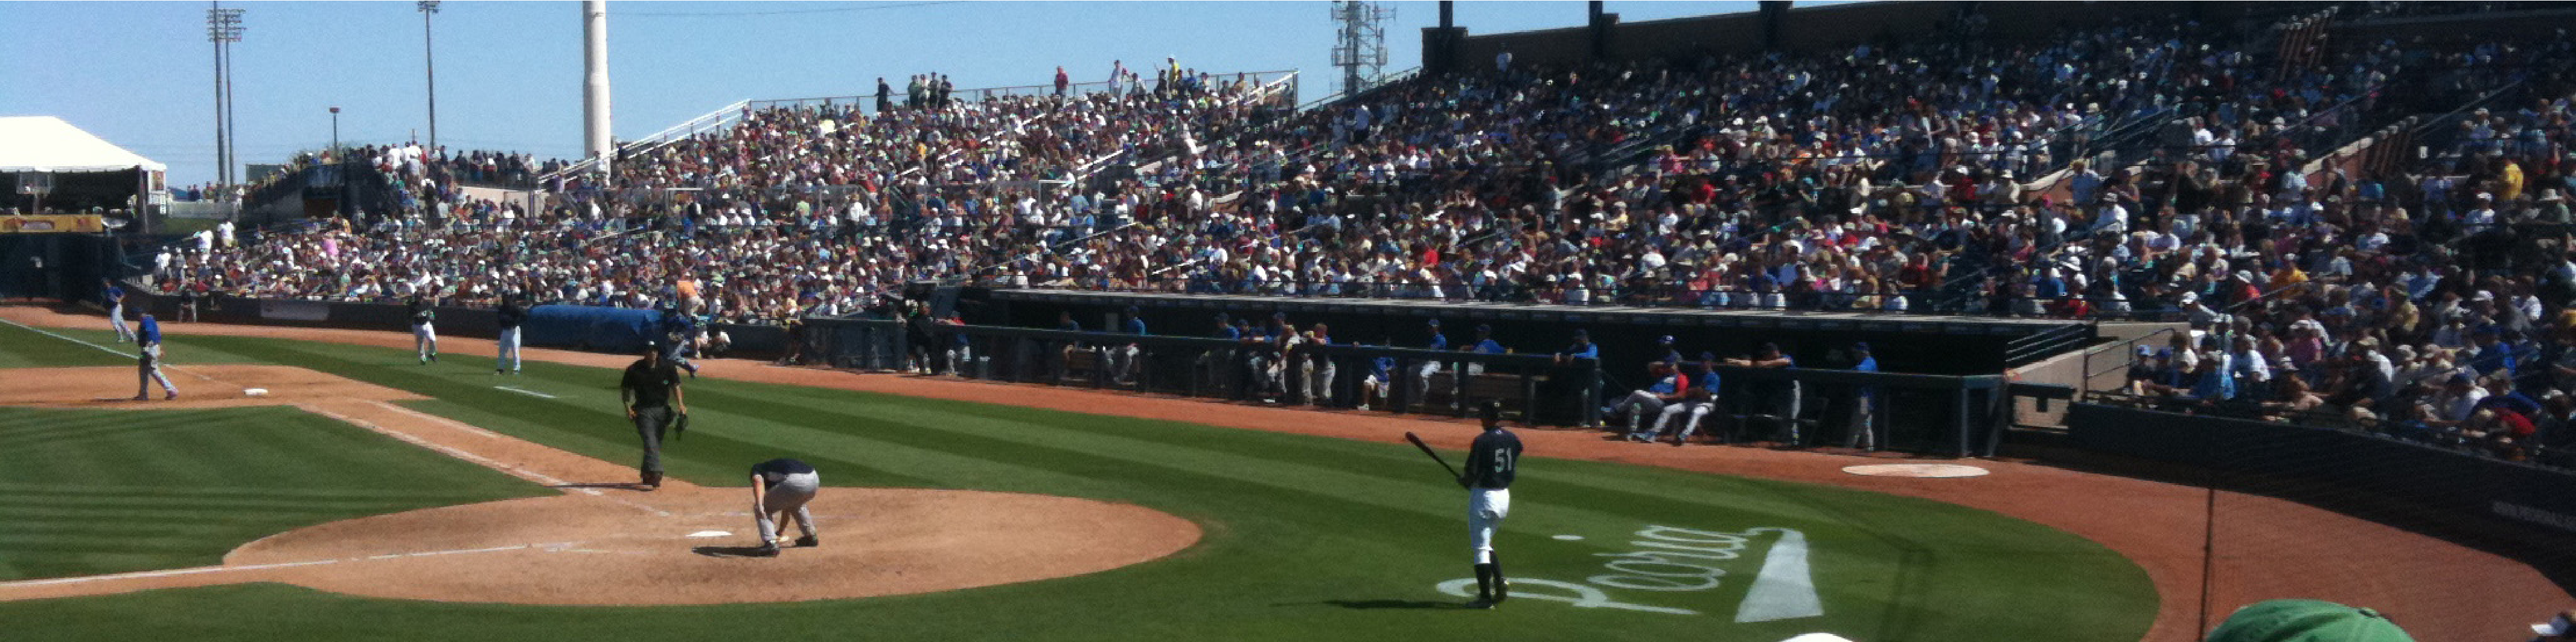
\includegraphics[width=\textwidth]{sampleteaser}
%   \caption{Seattle Mariners at Spring Training, 2010.}
%   \Description{Enjoying the baseball game from the third-base
%   seats. Ichiro Suzuki preparing to bat.}
%   \label{fig:teaser}
% \end{teaserfigure}

%%
%% This command processes the author and affiliation and title
%% information and builds the first part of the formatted document.
\maketitle

%%%%%%%%%%%%%%%%%%%%%%%%%%%%%%%%%%%%%%%%%%%%%%%%%%%%%%%%%%%%%%%%%%%%%%%%%%%%%%%%%%%%%%%%%%%%%%%%%%%
\section{Introduction}
\label{sec:intro}
%\vk{Finished with editing the text for now. I have elaborated some sections and also answered to your comments. Haven't removed your comments though, so you can find the unclear sections easily.
%Also added reference commands where ever needed. Only need to update bib file and plots.}
%\ggx{Reference are missing please fix!}

Latest years have witnessed a growing interest on the so called \emph{Deterministic Networks (DetNet)}. 
%Deterministic networks is part of time sensitive networking. 
In this type of networks, a bounded latency and zero packet loss is guaranteed to a set of priority flows. This can be achieved by mechanisms such as explicit bandwidth reservation, packet replication, and priority queuing~\cite{detnetrfc}. 
%The transmitter on the other end is also limited to a specific bandwidth. 
Although the type of mechanisms to be used in such networks are well described in the RFC and white-papers, there is no study in the literature about the possible algorithms that can be used at network layer in the context of Deterministic Networks. Currently, the major efforts are carried out at the link layer, where IEEE is trying to define a variant of the Ethernet protocol able to provide bounded latency and zero loss guarantees~\cite{tsn}~\cite{tsncisco}.

The most common approach to lower the packet loss probability to zero is to increase the size of buffers, as well as replicating the traffic on several independent links, while filtering the incoming traffic so as to make sure that no bandwidth allocation is ever violated (\cite{detnetrfc},~\cite{detnetwhitepaper}).
Limiting the transmitter to a specific bandwidth, and explicitly allocating resources in the network can be viewed as having virtually a separate link for each priority flow with a bandwidth equal to the reserved one. Such a strict reservation rule leads to under-usage of physical available bandwidth, since when the priority flows are inactive no other flow can take advantage of the unused bandwidth. 
Bandwidth sharing has always been a classical problem in networking. Numerous algorithms have been proposed for fair-sharing of bandwidth like RED-PD~\cite{redpd}, FRED~\cite{fred}, CHOKe~\cite{choke}. In our specific case, we aim at virtual bandwidth reservation (meaning, guaranteed maximum bandwidth) for priority flows in combination with fair sharing of the remaining bandwidth among non-priority flows. This makes it very complex and difficult to implement and make use of any of the algorithms proposed in the literature.
In this paper, we propose an algorithm inspired on the work of Addanki et al.~\cite{fairdrop}, which removes such waste of bandwidth, allowing other flows to use the bandwidth not consumed by DetNet flows.
In our algorithm, the concept of software virtual queues allows us to explicitly allocate resources to priority flows without increasing the number of physical buffers. 
While the bandwidth is shared by priority and non-priority (best effort) flows, we show that our modified fairdrop algorithm optimizes the usage of both unreserved and reserved-but-unused bandwidth by fairly sharing it among the non-priority flows. 
%Our algorithm acts a dropper before en-queuing a packet in the queue.

%In view of Deterministic Networking, our algorithm, inspired from X, eliminates the problem of increased number of packet buffers in the network and also eliminates the unused bandwidth problem by allowing the non-priority flows to use the bandwidth. The algorithm is also extremely simple to be implemented in software routers which are gaining popularity in the recent times.

In order to evaluate our proposal we implemented it in NS-3~\cite{ns3}, an industry standard network simulator. Such implementation represents a second contribution of this paper, since no DetNet scheduler is currently available for NS-3.\footnote{The NS-3 code will be made publicly available, however, it is not yet in a public repository because of the CoNEXT double blind submission policy.}  
%L: This can be stated in the NS-3 section: We introduce a new queue-disc which implements our algorithm under the traffic-control module of ns-3. 
We show by simulations, per-flow and total bandwidth usage, latency, queue length and packet loss.
We compare our solution with a network using native NS-3 FIFO queuing. 
The results show how our simple algorithm can easily guarantee explicit bandwidth reservation for priority flows in Deterministic Networks.

The remaining of the paper is organized as follows. In the following section (Sec.~\ref{sec:bandwidth}) we describe the essential components required for flow level bandwidth reservation. 
In Sec.~\ref{sec:algo} we present our algorithm, while in Sec.~\ref{sec:ns3} we briefly describe its  implementation in NS-3. Then, in Sec.~\ref{sec:simulations} we present the simulation results. Sec.~\ref{sec:conclusion} concludes the paper.




%%%%%%%%%%%%%%%%%%%%%%%%%%%%%%%%%%%%%%%%%%%%%%%%%%%%%%%%%%%%%%%%%%%%%%%%%%%%%%%%%%%%%%%%%%%%%%%%%%%
\section{Bandwidth reservation}
\label{sec:bandwidth}

In the context of bandwidth sharing, numerous algorithms from literature like RED-PD, CHOKE ~\cite{redpd},~\cite{choke} are stateless. This makes it difficult to achieve exact per-flow fair sharing of bandwidth. In a preliminary evaluation, we found that the statefull Fair-drop algorithm ~\cite{fairdrop} may achieve exact fair sharing of available bandwidth among concurrent flows. 
The concept of virtual queues introduced in this algorithm makes it easier for us to adopt some of the concepts into our algorithm to achieve per-flow bandwidth reservation and per-flow bandwidth sharing at the same time. The essential data structures of our algorithm are one global flow-table and two active-lists, one for each priority/non-priority set of flows. Fig.~\ref{fig:flowtable} shows the data structure definition in \texttt{C++}, as well as the logical organization and relation of both the flow-table and the two active-lists
we use. Hereafter we describe how they work.

%--------------------------------------------------------------------------------------------------
\begin{figure}[t]
    \centering
    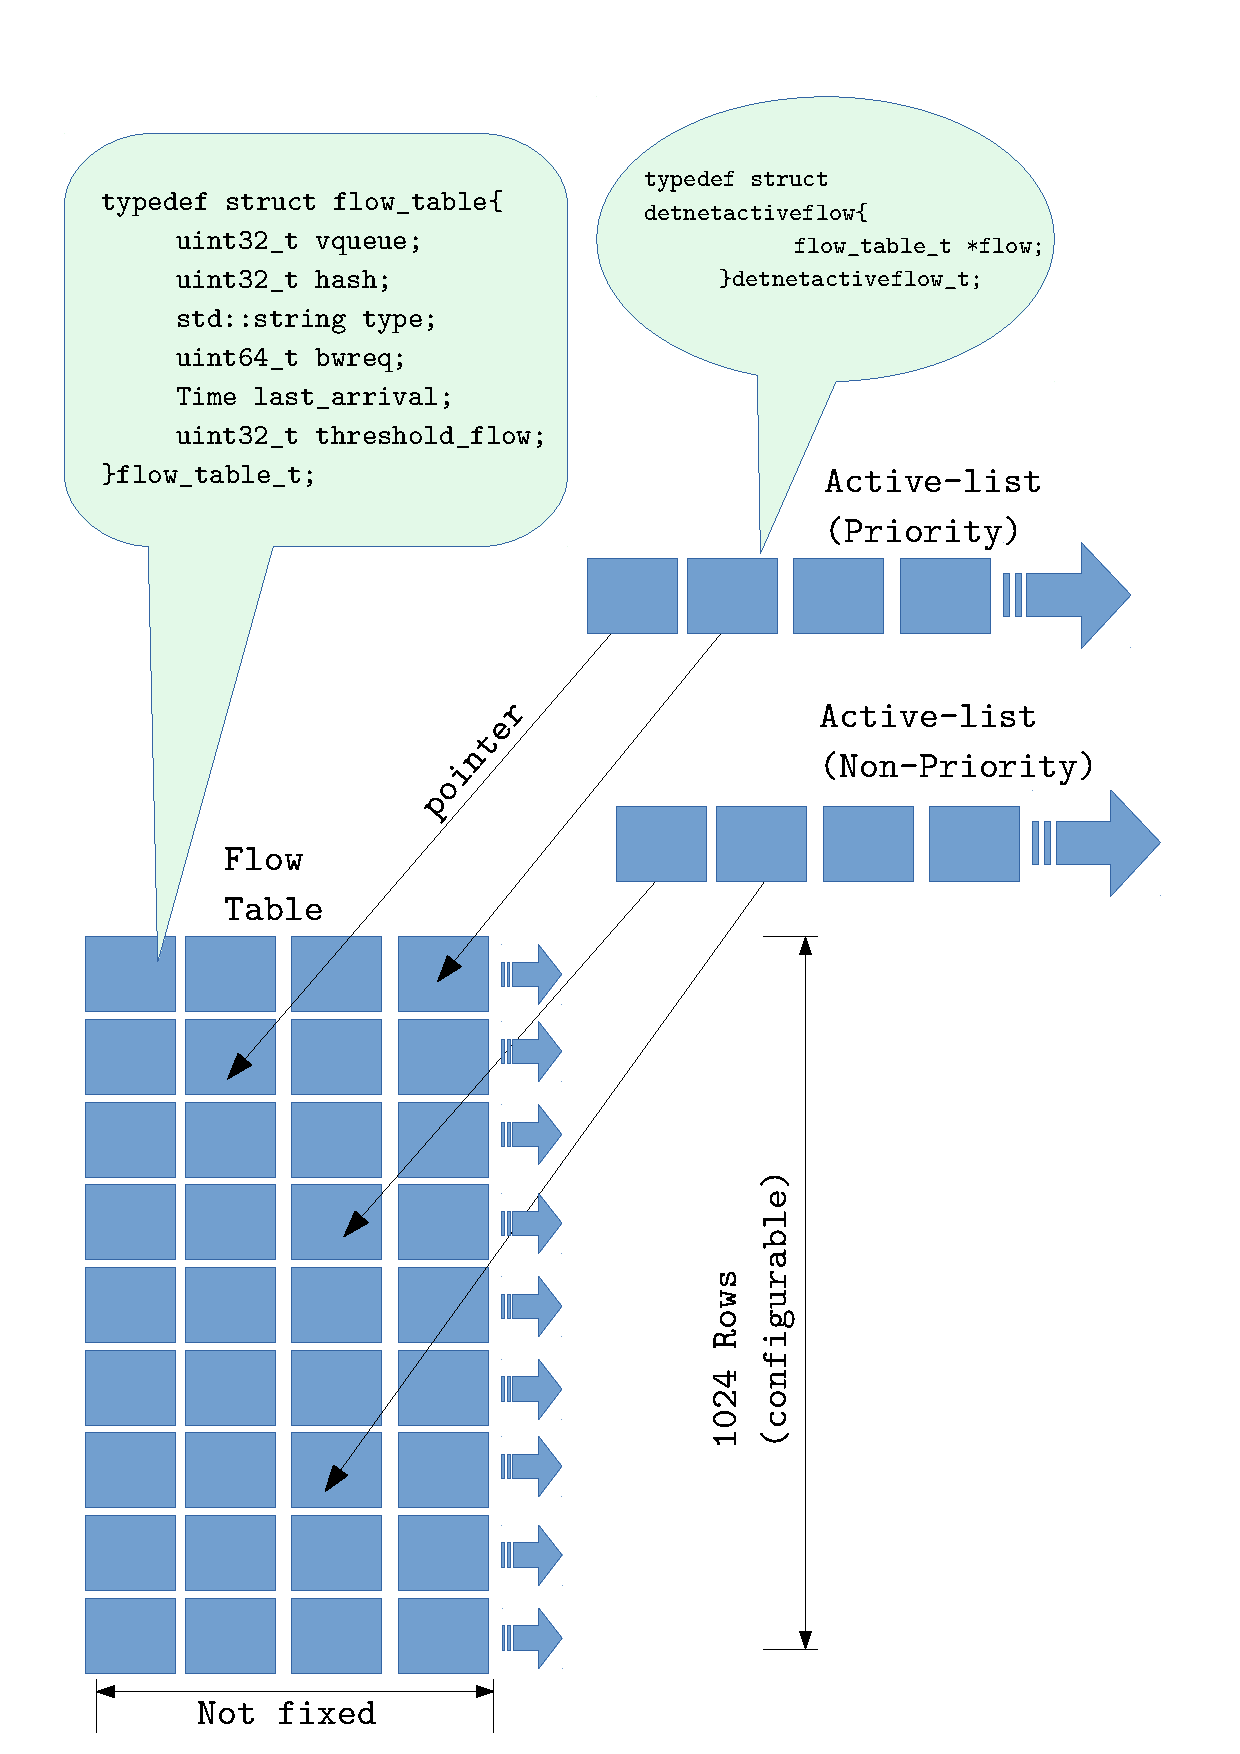
\includegraphics[width=0.7\linewidth]{figures/flowtable.pdf}
    \vspace{-3mm}
	\caption{Definition (in \texttt{C} language) and logical relation of the Flow-table and the active-lists data structures.}
	\label{fig:flowtable}
\end{figure}
%--------------------------------------------------------------------------------------------------

%%%%%%%%%%%%%%%%%%%%%%%%%%%%%%%%%%%%%%%%%%%%%%%%%%%%%%%%%%%%%%%%%%%%%%%%%%%%%%%%%%%%%%%%%%%%%%%%%%%
\subsection{Flow-Table}
\label{subsec:flowtable}

At the beginning, the flow-table is initialized with constant (\texttt{TABLESIZE}) number of rows and just one column. New arriving flows are classified in the flow-table based on the Receiver-Side Scaling (RSS) hash value~\cite{rssmicrosoft}~\cite{rsslinux}. RSS hash value is calculated by most of the hardware NICs in the recent times , hence, there is no overhead for the calculation of hash value. 

Flow classification is done by Algorithm~\ref{algo:flowclassification}. 
On packet arrival, the modulo of the RSS hash value with respect to the flow-table size (i.e., number of rows) is calculated, which gives the row index for the flow entry in the flow-table. 
Then a linear search is applied in the row to find the flow entry for the current packet. If there is no entry for this flow yet, a new flow entry is created at the end of the row.
When a new entry is created, the entry is initialized with the following values: packet-size, type (priority/non-priority), reserved bandwidth, last-arrival timestamp, virtual queue and threshold (the latter is related to algorithm described in Sec.~\ref{sec:algo}).

The scalability of the flow-table data structure comes from the fact that Deterministic Network is not expected to grow to a size comparable to the Internet. The most likely deployment big scenario is a big industrial plant, which remains to a limited-scale. In this scenario it is not hard to find a good hash function yielding a widely spaced range of hash values for the IP addresses in same or adjacent subnets. So the scale of flow-table collisions possible for this kind of network is expected to be low. This means that the per-row linear search, which is a time consuming operation, will be a rare event.  


%%%%%%%%%%%%%%%%%%%%%%%%%%%%%%%%%%%%%%%%%%%%%%%%%%%%%%%%%%%%%%%%%%%%%%%%%%%%%%%%%%%%%%%%%%%%%%%%%%%
\subsection{Active-Lists}
\label{subsec:lists}

Active-list is simply a list of all flows which have their virtual queue greater than zero (i.e., at least one packet is in the virtual queue). On packet arrival, and after flow classification, if the flow is found in the flow-table, the length of its virtual queue is checked. Note from Fig.~\ref{fig:flowtable} that each flow entry in the flow-table is the head of a virtual queue associated to that specific flow. 
If the arrival packet's virtual queue is zero, as shown in Fig.~\ref{fig:flowtable}, a pointer to the flow entry is added to the active-list corresponding to the type of the flow (priority or best-effort). If the virtual queue is greater than zero, it means that a pointer to the flow entry already exists in the active-list. 
So the active-list at any instant of time is a list of pointers to the flow entries in the flow-table whose virtual queues are greater than zero.
%\ggx{Can an active-list have several pointers to the same flow-entry? If yes please describe what it means. If no, please state why not!}
%\vk{the explanation above is clear to understand?}



%--------------------------------------------------------------------------------------------------
\begin{algorithm}[t!]
    \caption{\textbf{flow\_classify($pkt$)}}
    \label {algo:flowclassification}
    \begin{algorithmic}[1]
    \smaller 
    \STATE \textbf{Given:} pkt; TABLESIZE; flow\_table
    \STATE hash = pkt.gethash;
    \STATE mod = hash\%TABLESIZE;
    \FOR{every entry $i$ in flow\_table[mod]}
    \STATE flow\_entry=flow\_table[mod][i];
    \IF {hash == flow\_entry.hash}
    \STATE \textbf{return} flow\_entry;
    \ENDIF
    \ENDFOR
    \STATE create a new flow table entry flow\_table[mod][n+1];
%Space gaining avoid data structure filling
%    \STATE flow\_entry = flow\_table[mod][n+1];
%    \STATE flow\_entry.hash=hash
%    \STATE flow\_entry.vqueue=pkt.getSize();
%    \STATE flow\_entry.type=pkt.getType();
%    \STATE flow\_entry.last\_arrival=now();
%    \STATE flow\_entry.bwreq=pkt.Getbwreq();
%    \STATE flow\_entry.flow\_threshold=THRESHOLD;
%    \STATE \textbf{return} flow\_entry;
\end{algorithmic}
\end{algorithm}
%--------------------------------------------------------------------------------------------------



%%%%%%%%%%%%%%%%%%%%%%%%%%%%%%%%%%%%%%%%%%%%%%%%%%%%%%%%%%%%%%%%%%%%%%%%%%%%%%%%%%%%%%%%%%%%%%%%%%%
\section{Modified Fair Drop Algorithm}
\label{sec:algo}

Among the numerous concurrent flows, we have priority flows (PF) and non priority, best effort, flows (N\_PF). In the context of deterministic networks, we need to reserve bandwidth for priority flows while trying to achieve a maximum bandwidth utilization for the whole set of flows (priority and non priority flows). 
We achieve this by defining a maximum bandwidth utilization variable (\texttt{bwreq}) for each priority flow as shown in Fig.~\ref{fig:flowtable}. As long as the incoming flows bandwidth is less than such value, we can be certain that the flows experience zero packet loss. The un-utilized bandwidth (independent of total reserved bandwidth) is fairly shared among all the concurrent non-priority flows. 

At every packet arrival, after the usual processing of packet by the router, an enqueue operation for packet in the output buffer is attempted. The packet enqueue operation may fail when the output buffer is saturated. 
Our algorithm runs just before such enqueue operation, independent of the type of packet to be enqueued. The algorithm consists of two stages and is described hereafter.

%%%%%%%%%%%%%%%%%%%%%%%%%%%%%%%%%%%%%%%%%%%%%%%%%%%%%%%%%%%%%%%%%%%%%%%%%%%%%%%%%%%%%%%%%%%%%%%%%%%
%\ggx{My understanding is that the credit should be calculated upon "last transmitted packet". Or am I missing something?}
%\vk{Credit is calculated upon "packet arrival at enqueue operation". It doesn't matter whether the previous packet was dropped or not. The time difference multipled with bw is always expressing the number bits which can be added to virtual queues. We use the value of credit to decrement queues. This means that, as the queues are being emptied there will be more available capacity for the upcoming packets to be added to the virtual queues.}
%%%%%%%%%%%%%%%%%%%%%%%%%%%%%%%%%%%%%%%%%%%%%%%%%%%%%%%%%%%%%%%%%%%%%%%%%%%%%%%%%%%%%%%%%%%%%%%%%%%
\subsection {Stage-1}
\label{subsec:stage1}

Initially, the total available bandwidth (representing the credit in bits) is calculated by the difference between the arrival times of the current packet and the previous packet (of any type) multiplied with the total output bandwidth.
\begin{equation}
credit=(t_n - t_{n-1})*(BW_{output})\label{credit}
\end{equation}


%\ggx{The above is calculate for ALL packets or only for best effort non priority packets? Please state!}
Another credit is calculated for all the priority flows in the priority active-list. Priority-flow available bandwidth (priority-credit) is calculated by the difference between arrival time of current packet and last updated time of the same priority flow multiplied with its reserved bandwidth. 
\begin{equation}
priority\_credit_{pf}=(t_{npf}-t_{npf-1})*(BW_{reserved})\label{prioritycredit}
\end{equation}
%\ggx{The above is calculate for ALL packets or only for best effort non priority packets? Please state!}

First, the virtual queues of all the entries in the priority active-list are decremented by a value equal to the priority credit corresponding to the priority flow.
This expresses how much bandwidth they are allowed to consume which is bounded by a \texttt{THRESHOLD}.
If the virtual queue is decremented to zero, meaning that the priority credit of a priority flow is bigger than the amount of data to be transmitted present in the virtual queue, the flow is removed from the active-list. Otherwise the flow's active-list position is changed to the end of the list.
During this step, while decrementing the virtual queue of all active priority flows, the credit \emph{``actually''} used by the priority flows is cumulatively calculated in the \texttt{priority\_consumption} variable. The above operations are described in Algorithm~\ref{algo:stage11}.

%--------------------------------------------------------------------------------------------------
\begin{algorithm}[t]
    \caption{\textbf{BW Reservation (Stage-1)}}
    \label {algo:stage11}
    \begin{algorithmic}[1]
    \smaller
        \STATE \textbf{Given:} priority and non-priority active-lists, flowtable;
        \STATE $now$=time\_now();
        \STATE $priority\_consumption$ = 0;
%        \IF{size of priority active-list $>$ 0}  NOT NEEDE IF THE ACTIVE LIST IS EMPTY THE FOR IS NOT EXECUTED
            \FOR{every $flow$ in active-list}
                \STATE $\Delta t$ = $now$ - $flow.last\_arrival$;
                \STATE $priority\_credit$ = $\Delta t$ * $flow.bwreq$;
                \IF {$flow.vqueue$ $>$ $priority\_credit$}
                    \STATE $flow.vqueue$ -= $priority\_credit$;
                    \STATE $priority\_consumption$ += $priority\_credit$;
                    \STATE $flow.last\_arrival$ = now();
                    \STATE move the entry to the end of the active-list;
                \ELSE 
                    \STATE $priority\_consumption$ += $flow.vqueue$;
                    \STATE $flow.vqueue$ = 0;
                    \STATE remove the entry from the active-list;
                \ENDIF
            \ENDFOR
%        \ENDIF
    \end{algorithmic}
\end{algorithm}
%--------------------------------------------------------------------------------------------------

The value of \texttt{priority\_consumption} is used to calculate the amount of bandwidth that can be fairly shared by best effort traffic, following Algorithm\ref{algo:stage11}. Remaining-credit is calculated by subtracting \texttt{priority\_consumption} from \texttt{credit} and this is fairly divided among the entries of the active-list of non-priority flows. Similar to the previous step, the flow under consideration in the loop is moved to the end of the active-list, unless virtual queue reaches a zero value. In this last case, the flow is removed from the non-priority list and if such flow did not use its fair share of bandwidth, this is re-shared among the rest of the flows. The above operations are described in Algorithm~\ref{algo:stage12}.

%--------------------------------------------------------------------------------------------------
\begin{algorithm}[t]
    \caption{\textbf{Remaining BW fair sharing (Stage-1)}}
    \label {algo:stage12}
    \begin{algorithmic}[1]
        \smaller
        \STATE \textbf{Given:} priority and non-priority active-lists, flowtable, variables from Algorithm \ref{algo:stage11};

        \STATE $credit$ = $now$ - $Last Packet Arrival$;
        \STATE $remaining\_credit$ = $credit$ - $priority\_consumption$;
% NOT NEEDED        \IF{$remaining\_credit > 0$ \&\& Size of non-priority active-list $> 0$}
        \WHILE {Size of non-priority active-list $> 0$ \&\& $remaining\_credit > 0$}
            \STATE $fairbw$=$remaining\_credit$/Size of non-priority active-list; 
            \STATE $remaining\_credit$ = 0;
            \FOR {each $flow$ in non-priority active-list}
                \IF {$flow.vqueue$ $>$ $fairbw$}
                    \STATE $flow.vqueue$ -= $fairbw$;
                    \STATE move the entry to the end of the active-list;
                \ELSE
                    \STATE $remaining\_credit$ += $fairbw$ - $flow.vqueue$;
                    \STATE $flow.vqueue$ = 0;
                    \STATE remove the entry from active-list;
                \ENDIF
            \ENDFOR
        \ENDWHILE
%\ENDIF

\end{algorithmic}
\end{algorithm}
%--------------------------------------------------------------------------------------------------


%%%%%%%%%%%%%%%%%%%%%%%%%%%%%%%%%%%%%%%%%%%%%%%%%%%%%%%%%%%%%%%%%%%%%%%%%%%%%%%%%%%%%%%%%%%%%%%%%%%
\subsection {Stage-2}
\label{subsec:stage2}

%\ggx{I think this section should be re-written. There are several unclear points. 
%1. Nothing is said about threshold w.r.t. to respecting the  bandwidth allocation.
%2. is not clear what is the relation with previous. make examples. when is a packet dropped? When is put in the output queue.
%3. it is unclear when the packet is actually sent out. Pleas elaborate more on this part.}

After Stage-1, the current packet is inspected and the flow-entry in the flow-table, corresponding to the current packet is found using Algorithm~\ref{algo:flowclassification}.

If the sum of packet size and it's virtual queue is greater than a THRESHOLD, the packet is exceptionally dropped before the enqueue operation. If the sum is less than a THRESHOLD, the virtual queue can be zero or greater than zero. Only if the virtual queue is zero, a pointer to the packet's flow-entry in the flow-table is added to active-list corresponding to type of the packet. Finally, the packet size is added to the virtual queue and sent for enqueue operation.



%\vk{This is supposed to be like a conclusion to the entire section. "By this" i mean to say by using this kind of stage-1 and then stage-2 to share the bw, we make sure that priority flows are always getting their reserved bw requirement.}
%\ggx{The following sentence is unclear. What do you mean by "by this" ?? As far as I understand the priority is given in stage one when first credit consumption for priority flows is calculated before the best effort. NO?}
By serving the priority flows first in the stage-1 and then allowing the non-priority flows to use the remaining bandwidth in stage-2, we make sure that the priority flows are able to use their reserved bandwidth. As a matter of fact, if the transmitter obeys the limit of reserved bandwidth, we observe close to zero packet loss for all priority flows. Thus we achieve a combination of bandwidth-reservation and bandwidth-fair-sharing in deterministic networks.




%%%%%%%%%%%%%%%%%%%%%%%%%%%%%%%%%%%%%%%%%%%%%%%%%%%%%%%%%%%%%%%%%%%%%%%%%%%%%%%%%%%%%%%%%%%%%%%%%%%
\section{NS-3 Implementation}
\label{sec:ns3}

We introduced a new queue ``BW\_RESV'' under the traffic-control layer~\cite{traffic-control} of NS-3. All the calls to the enqueue operation of this queue will run our algorithm before attempting to enqueue a packet.
%\ggx{You need to describe what a queu dis is. Also, can you elaborate a bit more about the modules you changed and the code you wrote?} \vk{Explaining this can take up a lot of space. The reference above ~\cite{traffic-control} documentation of ns3 https://www.nsnam.org/doxygen/group\_\_traffic-control.html#details this will give enough information} The algorithm is implemented in the en-queuing operation of this queue. 
%Traffic generation is not relevant here: We use On-off application of ns-3 as packet-generator. 
%\ggx{Not sure is the right way to put it. You should rather state that for the sake of lightweight implementation you tag the packet explicitly. It may not be conform of reality, but this is just to simplify the flow identification. Also you have to describe what did you use as RSS function or how you created an equivalent.} 
For the sake of simplicity of network configuration with bandwidth reservation and type of packets, we tag the transmitted packets. The tag is of the format ``XXXXKbps Y''. Here X are 4 numeric digits for the reserved bandwidth/bitrate, Y is the type of flow where D corresponds to priority flow and O corresponds to non-priority flow (for example ``1000kbps D''). When a packet arrives at ``BW\_RESV'' queue for the first time, the packet tag is read to identify the type of the flow and it's bandwidth requirement. We use default ns3 configuration for accessing hash value of a packet which is calculated based on murmur3 hashing algorithm~\cite{ns3hash}~\cite{murmur3}.




%--------------------------------------------------------------------------------------------------
\begin{algorithm}[t]
    \caption{\textbf{On packet arrival (Stage-2)}}
    \label {algo:stage2}
    \begin{algorithmic}[1]
        \smaller
        \STATE \textbf{Given:} packet's flow entry $flow$, $packet\_size$;
        \IF {$flow.vqueue$ $>$ $THRESHOLD$}
            \STATE drop();
            \STATE exit();
        \ELSE
            \IF{$flow.vqueue$ == 0}
                \STATE add the flow to the corresponding active-list by type;
            \ENDIF
            \STATE $flow.vqueue$ += $packet\_size$;
            \STATE $flow.last\_arrival$ = now();
            \STATE enqueue();
        \ENDIF
\end{algorithmic}
\end{algorithm}
%--------------------------------------------------------------------------------------------------


% \begin{figure}[ht]
% 	\begin{center}
% 		\includegraphics[width=0.50\textwidth]{figures/topology.pdf}
% 		\caption{Topology}\label{fig:topology}
% 	\end{center}
% \end{figure}


\section{Simulations}
\label{sec:simulations}

In this section we first present the simulation set up we used for evaluation, then we showcase the results that we obtained.

\subsection{Simulations Set Up}
\label{subsec:simsetup}

We use a simple network with 4 hosts and 2 routers. Two hosts are connected to each router and the two routers are connected to each other via a single bottleneck link.
%, as shown in Fig. [\ref{fig:topology}]. 
The hosts on one router generate traffic, while hosts on the other router act as sinks. 
All the links in the network are 30 Mbps except the link between the routers, which is 10 Mbps.
%The input link of Router-1 is configured high so that the output link becomes a bottleneck when there is a heavy traffic at the input. 
%The router attached to the traffic generating hosts uses either a traditional FIFO queue or our BW\_RESV queue implementing our algorithm.



During simulations, we generate 5 flows, all with a packet size of 1000 bytes, out of which 3 flows are priority flows and 2 flows are non-priority flows. The \texttt{THRESHOLD} parameter in our algorithm is set to 10 times the maximum packet size. All the priority flows are configured with bandwidth reservation of 2000Kbps. Non-priority flows are given flow-id 1, 2 and the priority flows are given flow-ids 3, 4 and 5. Transmission of these flows start at times (in seconds) at t=1, t=5, t=8, t=12, t=16 in the order of their flow-ids.
Non-priority flows i.e flows 1 and 2 are both generated at 5000Kbps. Priority flows i.e flows 3, 4 and 5 are generated at 1000Kbps, 5000Kbps and 2000Kbps respectively while they all have a reservation of 2000Kbps.  %\ggx{why this? I suppose you want to show that even if we generate 1Mbps what flows thorugh is just what has been reserved.} \ggx{BTW somewhere in the paper you must state that bandwidth reservation is done by configuration. } \vk{This is explained in the last paragraph of this subsection} 
 With this traffic, we have no congestion in any of the links, except the 10Mbps link, which is the single link between the two routers. We run simulations generating network traffic as stated above with our $BW\_RESV$ queue and a $FIFO$ queue to make a comparison and show that we can achieve bandwidth reservation and fair sharing at the same time.

This configuration is used for all the experiments except \ref{exp:packetloss} where we show that we can achieve zero packet-loss when the priority flows respect the bandwidth reservation policy. The above configuration is used on purpose to show that even though some of the priority flows exceed in throughput w.r.t their bandwidth reservation, our algorithm allows them to use only the configured reserved bandwidth.

%\ggx{what is the threshold value sued in the simulations?} \vk{updated in the text above.There is also an explanation about threshold values that can be used, at the end of 5.2.3 section}

%\ggx{Replot figures for B\&W printing} \vk{done. I had to change the experimental scenario inoder to plot for B\&W printing. With 12 flows, the plots become too congested in space when i use lines and points to plots}

\subsection{Simulations Results}
\label{subsec:simsetup}

\subsubsection{Throughput}
We measured throughput of flows at the output of first Router (with bottleneck link), so as to verify that bandwidth reservation is respected and best effort traffic can fairly share the residual bandwidth.
Fig.~\ref{fig:rx_detnet} shows what has been obtained.
We can observe that between t=1 and t=8, there is no congestion, and the flows present does not experiences drops. 
%\ggx{should provide detailed description for slots 0->1, 1->2, 2->3 and then state that everything change in the same way.}
Starting from t=8, when the non-priority flow-1 (flow-id 3) starts, we see that priority flow-1 is given exactly the configured bandwidth reservation i.e 1000Kbps and the remaining bandwidth is shared by the two non-priority flows. When new priority flows are added (for example at t=12), the remaining bandwidth to be shared by non-priority flows reduces as the new priority flow is allowed to use its configured reserved bandwidth. The same pattern continues in the graph. In this case, the difference between flow's input and output throughput is entirely due to dropping of packets by the algorithm based on the reservation and sharing configurations. We can also see that, although priority flow-2 (flow-id 4) transmits at 5000Kbps, it is only allowed to use 2000Kbps which is it's bandwidth reservation.

%When an additional priority flow is introduced, the remaining bandwidth reduces and it is fairly shared by the two non-priority flows.

%--------------------------------------------------------------------------------------------------
\begin{figure}[t]
	\centering
	\includegraphics[width=0.7\linewidth]{plots/rx_detnet_new.pdf}
    \vspace{-3mm}
	\caption{Output rate per flow when bwresv queue is activated on the router with bottleneck link.}
	\label{fig:rx_detnet}
\end{figure}
%--------------------------------------------------------------------------------------------------

Fig.~\ref{fig:rx_fifo} shows a simulation with first router is configured with $FIFO$ queue at the output. 
This scenario can be compared to best-effort service. We see that there is no specific pattern in how the output bandwidth is shared. %\ggx{Elaborate more...} \vk{Sorry it is supposed to be ``no specific pattern'' instead of ``specific pattern''} 
Most importantly, the priority flows don't always get the reserved bandwidth at the output due to the excessive usage of bandwidth by non-priority and other priority flows.

%--------------------------------------------------------------------------------------------------
\begin{figure}[t]
	\centering
	\includegraphics[width=0.7\linewidth]{plots/rx_fifo_new.pdf}
    \vspace{-3mm}
	\caption{Output rate per flow with fifo queues at the output of the router with bottleneck link.}
	\label{fig:rx_fifo}
\end{figure}
%--------------------------------------------------------------------------------------------------



\subsubsection{End-to-End Delay}
The average end-to-end Delay has been measured by simulations using flow-monitor module~\cite{flowmonitor} of NS-3. 
Fig.~\ref{fig:delay_all} shows a simulation with ``FIFO'' queues at Router's output. We can observe that the average delay remains very low until the link is congested and reaches a maximum when the queue is saturated. 

%--------------------------------------------------------------------------------------------------
% \begin{figure}[t]
%     \centering
%     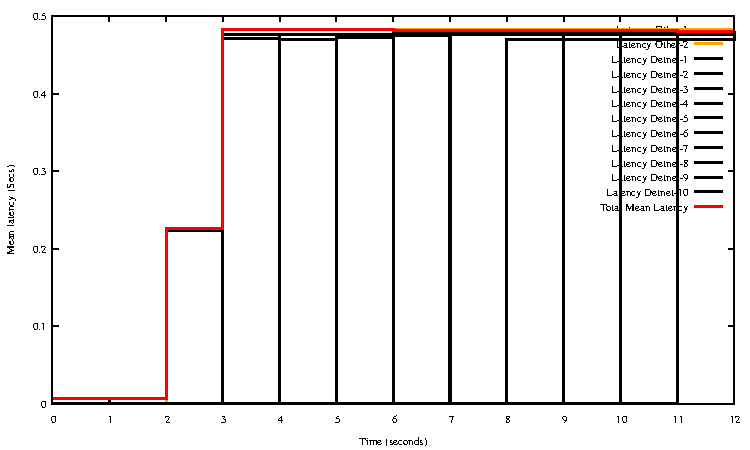
\includegraphics[width=0.7\linewidth]{plots/delay_fifo.pdf}
%     \vspace{-3mm}
% 	\caption{Average end-to-end latency when using FIFO output queue.}
% 	\label{fig:delay_fifo}
% \end{figure}
%--------------------------------------------------------------------------------------------------


Fig.~\ref{fig:delay_all} also shows the same simulation when our ``BW\_RESV'' queue is installed at router's output and configured with different values of \texttt{THRESHOLD}. 
We see that the average delay is relatively very low. Although, there is a small incremental pattern when new priority flows are added. This could be a result of choice of ``THRESHOLD'' of algorithm which allows a short duration of bursty traffic (exceeding the throughput limit) to pass resulting in increased number of packets in the real queue. This effect might also include the overhead of measurement or the per-flow overhead of algorithm or a combination of both. We leave it for future work to investigate this effect. %\ggx{Could it be that while vqueues are almost always empty, the actual output buffer can have up to a number of packets in the queue that is equal the number of detnet flows?} \vk{I have written some explainations about threshold and other possible effects in this section and also the next section.}
The most-important aspect of deterministic networks is bounded latency. We can clearly see from simulations that our algorithm can be configured properly to achieve a specific bounded latency.

%--------------------------------------------------------------------------------------------------
\begin{figure}[t]
	\centering
	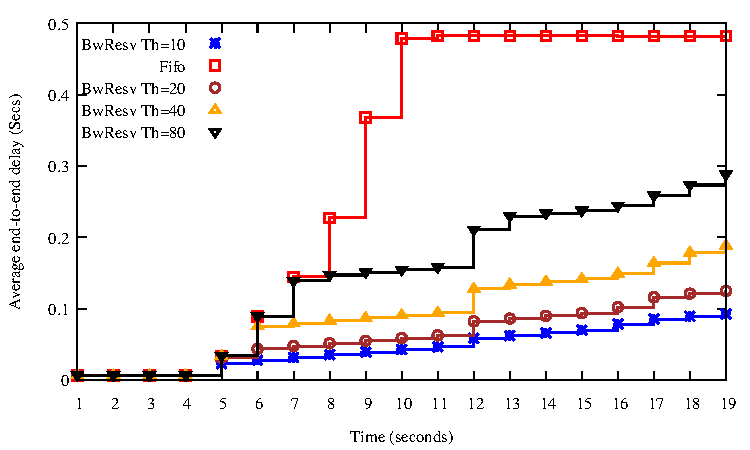
\includegraphics[width=0.7\linewidth]{plots/delay_all.pdf}
    \vspace{-3mm}
	\caption{Mean end-to-end latency in the cases when fifo is installed / bw\_resv queue is installed with different values of threshold.} 
	%\ggx{There is not best effort traffic here? Why?}} \vk{just above}
	\label{fig:delay_all}
\end{figure}
%--------------------------------------------------------------------------------------------------


% \begin{figure}[ht]
% 	\begin{center}
% 		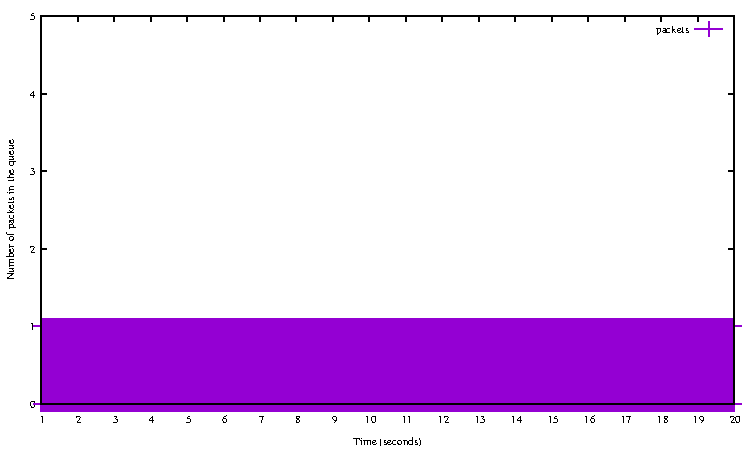
\includegraphics[width=0.50\textwidth]{plots/pkt_detnet.pdf}
% 		\caption{Mean Queue length of bw\_resv queue installed at the output of router-1}\label{fig:pkt_detnet}
% 	\end{center}
% \end{figure}
% \begin{figure}[ht]
% 	\begin{center}
% 		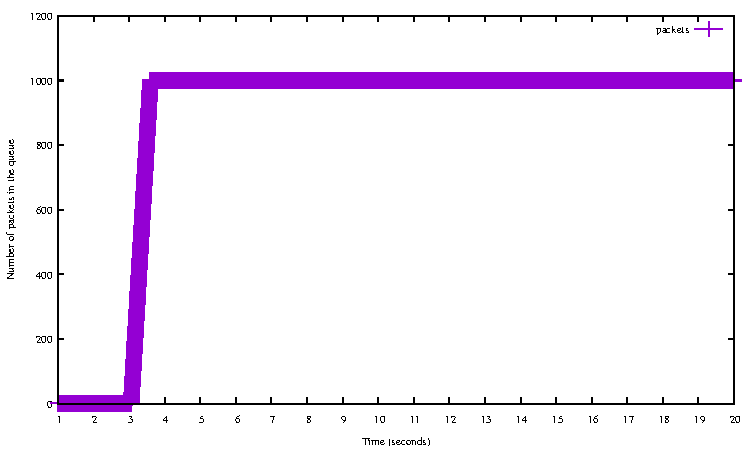
\includegraphics[width=0.50\textwidth]{plots/pkt_fifo.pdf}
% 		\caption{Mean Queue length of fifo queue installed at the output of router-1}\label{fig:pkt_fifo}
% 	\end{center}
% \end{figure}


\subsubsection{Queue Length}

We also measured the number of packets in the output queue of the first router at each packet arrival. In this section we run the same experiment as the previous section with flow average throughput being the same, with Constant Bitrate (CBR) and Poisson traffic, while varying the THRESHOLD parameter in our algorithm. We see that, in the case of FIFO queue from Fig~\ref{fig:pkt_all}, the number of packets in the queue is close to zero until saturation, and starting from t=5, the queue length slowly reaches to full capacity and starts to drop packets. The increase in the queue length is one of reasons why the average delay of packets reaches a maximum due to the waiting time in the queue. 

%--------------------------------------------------------------------------------------------------
\begin{figure}[t]
	\centering
	\includegraphics[width=0.7\linewidth]{plots/pkt_all_new.pdf}
    \vspace{-3mm}
	\caption{Mean Queue length at the output of router-1}
	\label{fig:pkt_all}
\end{figure}
%--------------------------------------------------------------------------------------------------

We avoid this problem by making drop decisions at each packet arrival to avoid congestion in the output queue. This is done while ensuring the bandwidth reservation and sharing configurations. As a result, we see that the queue length stays close to zero. A higher value of THRESHOLD parameter helps to protect the flows with bursty patterns. Although the queue length increases with higher thresholds at heavy loads, this is entirely left as administrator's choice between mean-latency and packets loss probability. Fig~\ref{fig:pkt_all} also shows plots for extreme cases with threshold parameter set to greater than 20 times maximum packet size. Since the algorithm runs at every packet arrival, thresholds such high are extremities. For instance, let Y bits/sec be the throughput of a priority flow which is greater than X bits/sec, it's reserved bandwidth. With a higher threshold value say Z bits, the configuration would allow higher throughput to pass for Z/(Y-X) seconds. When Z is large, the time for which we allow a higher throughput of the flow to pass will increase resulting in temporary saturation of the queue.
%\ggx{Explicitly state that the figure is useless because queues are always empty....} 

%--------------------------------------------------------------------------------------------------
\begin{figure}[t]
  \centering
  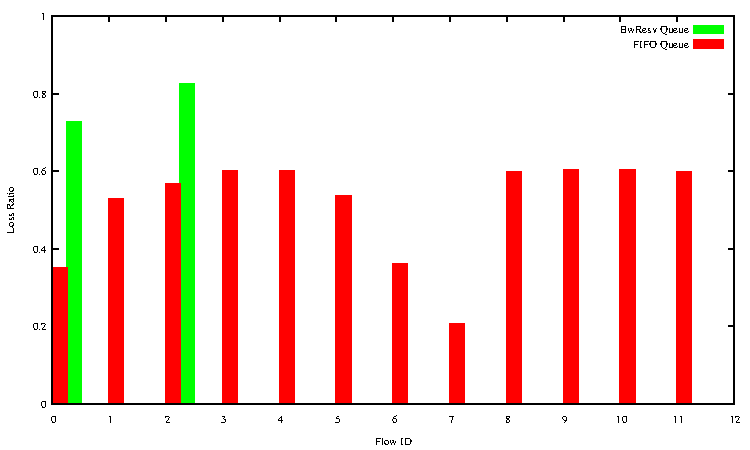
\includegraphics[width=0.7\linewidth]{plots/loss.pdf}
  \vspace{-3mm}
  \caption{Overall packet loss}
  \label{fig:loss}
\end{figure}
%--------------------------------------------------------------------------------------------------

\subsubsection{Packet Loss}
\label{exp:packetloss}
In this experiment, we show that we can achieve zero packet loss when priority flows respect their bandwidth reservation limit.
We run experiments with 5 flows consisting of 3 priority flows, 2 non-priority flows and the bottleneck link is configured at 10Mbps. Priority flows (flow-ids 3, 4 and 5) transmit at 1000Kbps, 5000Kbps and 1500Kbps respectively while they all have a bandwidth reservation of 2000Kbps. The non-priority flows (flow-ids 1 and 2) transmit at 10000Kbps. From the traffic configuration we can see that flow-id 4 violates its bandwidth reservation limit. All the flows start to transmit at times exactly same as in the previous experiments. When all the flows are in progress, they intersect at the first router, with one output link of 10Mbps. As we can notice immediately, the output link is rapidly saturated.%\ggx{what do you mean?} \vk{Just want to stress that the link is saturated and is at high load}. 
In this scenario, we run experiments to check the overall packet loss experienced by the flows during the whole experiment. We can see from Fig.~\ref{fig:loss} that the priority flows which respect the bandwidth reservation limit have an exact zero packet loss as expected. We see that even though a flow is categorized as a priority flow it experiences packet loss when it violates the bandwidth reservation limit. From Fig.~\ref{fig:loss}, we see 61\% packet loss for the priority flow transmitting at 5000Kbps which has only 2000Kbps reservation. As expected, we see packet loss for non-priority flows as we have priority flows in progress. On the other hand, we can see that there is a heavy packet loss for all the flows when using FIFO queue. 


%%%%%%%%%%%%%%%%%%%%%%%%%%%%%%%%%%%%%%%%%%%%%%%%%%%%%%%%%%%%%%%%%%%%%%%%%%%%%%%%%%%%%%%%%%%%%%%%%%%
\section {Conclusions}
\label{sec:conclusion}

In this paper, we proposed a modified fair drop algorithm, which can be implemented very easily in the context of Deterministic Networking. 
Our first contribution is the adaptation of this type of algorithm to the DetNet uses case, in order to achieve bandwidth reservation and fair bandwidth sharing.
As a second contribution, we implemented DetNet module for NS-3. The latter was insofar completely lacking a module allowing to perform DetNet simulations. 
Leveraging on the NS-3 implementation, we did show that our algorithm can achieve zero packet loss by bandwidth reservation and maximizes the utilization of unused bandwidth by fairly sharing it among the non-priority flows.
As future work we plan to evaluate our algorithm in more complex scenarios, while introducing other DetNet features, like traffic duplication.



%%
%% The next two lines define the bibliography style to be used, and
%% the bibliography file.
\bibliographystyle{ACM-Reference-Format}
\bibliography{references}

%%
%% If your work has an appendix, this is the place to put it.
%\appendix

\end{document}
\endinput
%%
%% End of file `sample-authordraft.tex'.
